\subsection{Macrobenchmarks}
\label{macro}

\begin{figure*}[t]
        \centering
        \begin{subfigure}[b]{0.45\textwidth}
                \centering
                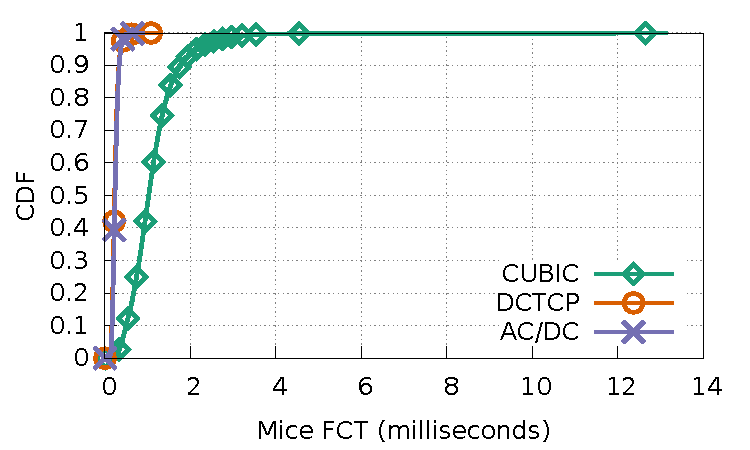
\includegraphics[width=\textwidth]{figures/macro_benchmarks/macro_4stride/stride4_mice16KB_fct.pdf}
                \caption{mice flows}
                \label{macro_4stride_mice_fct}
        \end{subfigure}
        \begin{subfigure}[b]{0.45\textwidth}
                \centering
                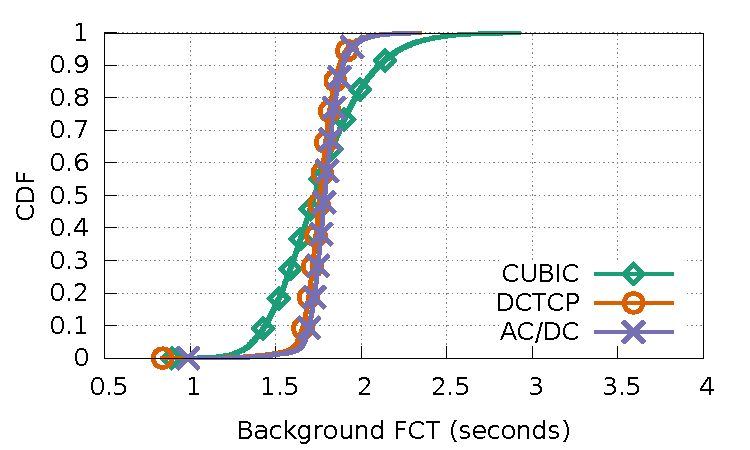
\includegraphics[width=\textwidth]{figures/macro_benchmarks/macro_4stride/stride4_big512MB_fct.pdf}
                \caption{background flows}
                \label{macro_4stride_background_fct}
        \end{subfigure}
        \caption{CDF of both mice flows and background flows' FCTs in concurrent stride workload.
                For mice flows, median (DCTCP reduce by 77\%, Ours 76\%),
                99th percentile (DCTCP 84\%, Ours 85\%),
                99.9th percentile (DCTCP 91\%, Ours 93\%).}
        \label{macro_4stride_fct}
\end{figure*}

\begin{figure*}[t]
        \centering
        \begin{subfigure}[b]{0.45\textwidth}
                \centering
                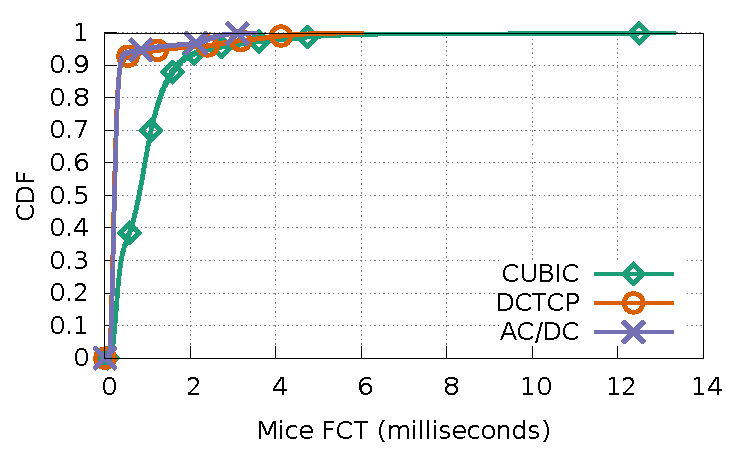
\includegraphics[width=\textwidth]{figures/macro_benchmarks/shuffle_17hosts/shuffle_mice16KB_fct.pdf}
                \caption{mice flows}
                \label{macro_shuffle_mice_fct}
        \end{subfigure}
        \begin{subfigure}[b]{0.45\textwidth}
                \centering
                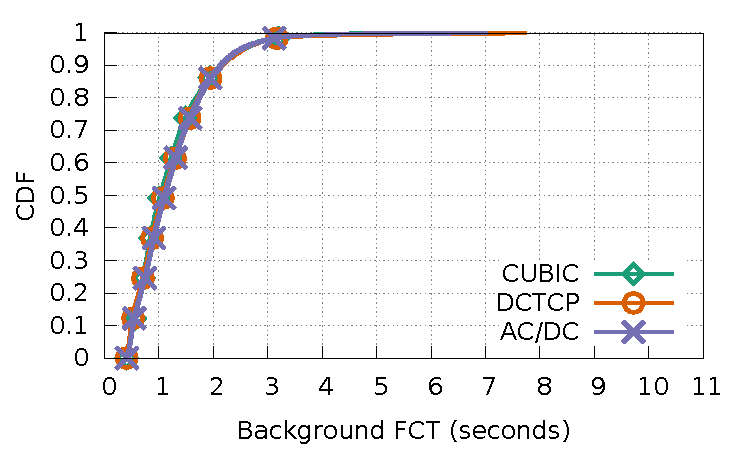
\includegraphics[width=\textwidth]{figures/macro_benchmarks/shuffle_17hosts/shuffle_big512MB_fct.pdf}
                \caption{background flows}
                \label{macro_shuffle_background_fct}
        \end{subfigure}
        \caption{CDF of both mice flows and background flows' FCTs in shuffle workload.
                For mice flows, median (DCTCP reduces by 72\%, Ours 71\%),
                99th percentile (DCTCP 20\%, Ours 48\%),
                99.9th percentile (DCTCP 55\%, 73\%).}
        \label{macro_shuffle_fct}
\end{figure*}

\begin{figure*}[t]
        \centering
        \begin{subfigure}[b]{0.45\textwidth}
                \centering
                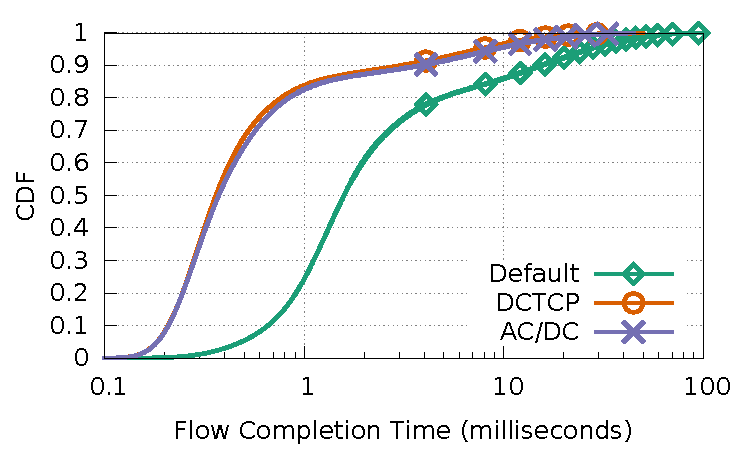
\includegraphics[width=\textwidth]{figures/macro_benchmarks/trace-driven/trace_driven_workload_dctcp_senders5.pdf}
                \caption{web-search workload}
                \label{trace-driven-searching-fct}
        \end{subfigure}
        \begin{subfigure}[b]{0.45\textwidth}
                \centering
                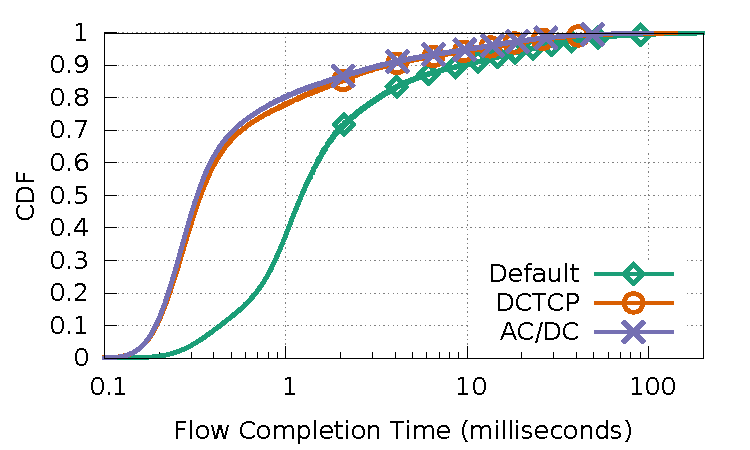
\includegraphics[width=\textwidth]{figures/macro_benchmarks/trace-driven/trace_driven_workload_conga_senders5.pdf}
                \caption{data-mining workload}
                \label{trace-driven-data-mining-fct}
        \end{subfigure}
        \caption{CDF of mice flow's (<10KB) FCT in trace-driven workloads.
                Y-axis is cut at 99.9\% for clarity.
                Web searching workload: median (DCTCP reduces by 77\%, Ours: 76\%),
                99th percentile (DCTCP: 65\%, Ours: 57\%),
                99.9th percentile (DCTCP: 50\%, 55\%).
                Data mining workload: median (DCTCP 72\%, Ours 73\%),
                99th percentile (DCTCP: 41\%, Ours: 48\%),
                99.9th percentile (DCTCP: 36\%, Ours: 53\%).}
        \label{macro-trace-driven-fct}
\end{figure*}




To better understand LiquidSwitch's benefits for real TCP applications, 
we wrote TCP
client/server programs to measure flow completion times.
First, TCP clients establish long-lived TCP connections with TCP servers. 
Then each client program sends messages with proper sizes and intervals, 
either sampled from a distribution (trace-driven) or take user-specified parameters.

\tightparagraph{Concurrent stride workload}
First, we run a concurrent stride workload---17 servers are attached to a single 10Gbps switch.
Each server $i$ sends 512MB data to servers [$i+1$, $i+4$]\%17.
In other words, each server sends 4 concurrent flows and receives 4 concurrent flows.
These elephant flows are used to emulate the background traffic.
At the same time, Each server $i$
builds a long-lived TCP connection with server $(i+8)\%(number\_of\_servers)$ and sends short messages
of size 16KB every 100 millisecond. The experiments for each setting last for 10 mintues.
Flow completion times for both mice flow (16KB) and background flow (512MB) are shown 
in Figure~\ref{}. For mice flows, at 50$^{th}$ percentile (i.e., median), DCTCP and \acdc{} 
reduces flow completion time by 77\% and 76\% respectively. 
At 99$^{th}$ percentile, DCTCP and \acdc{} reduces flow completion time by 84\% and 85\% respectively. 
At 99.9$^{th}$ percentile, DCTCP and \acdc{} reduces flow completion time by 91\% and 93\% respectively.
For background flows, DCTCP and \acdc{} offer similar completion times. 
Default has longer tail completion time because of CTCP and \acdc{} have better throughput fairness.


\tightparagraph{Shuffle workload}
Second, we run a shuffle workload. Background flow is 512MB, mice flow is 16KB, mice flow is sent every
100 msec. We run shuffle workload for 30 runs.
We show both the background and mice flow's flow completion times.

\tightparagraph{Trace-driven workloads}
Finally, we do trace-driven workloads. We wrote customer TCP client/server programs.
Each server starts 5 concurrent client processes and server processes.
Each client process builds a long-lived TCP connection with every other server in this testbed.
The flow sizes are sampled from two empirical workloads---web-search workload~\cite{alizadeh2011data}
and data-mining workload~\cite{greenberg2009vl2,alizadeh2014conga} which is more heavier at the tail.
For each experiment setting, we run it for 10 minutes and we gathered the flow completion times (FCTs) of tens of millions of flows.
